\documentclass[M3_Night5_Solutions]{subfiles}

\IfSubStr{\jobname}{\detokenize{Solutions}}{\toggletrue{solutions}}{\togglefalse{solutions}}

\fancypagestyle{firstpage}

{\rhead{Night 5 \linebreak \textit{Version: \today}}}

\title{Night 5: Polar LIDAR Express}
\author{Quantitative Engineering Analysis}
\date{Spring 2019}

\begin{document}

\maketitle
\thispagestyle{firstpage}

\solution{\textbf{Note: The Matlab Script used to make the solution plots is \href{https://drive.google.com/file/d/1tITJihd8XavPmY8HPXIAIbZano3iHPhz/view?usp=sharing}{here}.}}

\section{LIDAR in Polar and Cartesian Coordinates}
\subsection{Laser Scanner}

\begin{marginfigure}
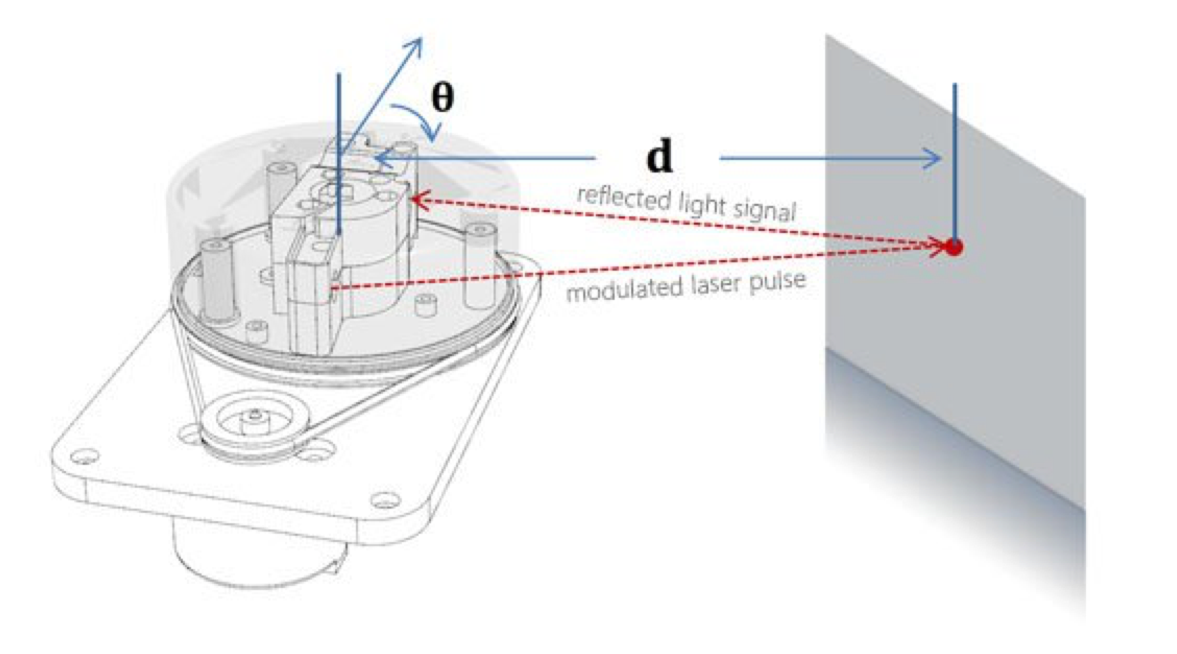
\includegraphics[width=2in]{figs/mechanism}
\caption{A schematic of the Neato's laser scanner.  Due to the relative position of the emitter and detector, the position of the reflected light changes  predictably as a function of $d$.  The laser scanner spins with a rate of $5$Hz.  The angle of the scanner is denoted as $\theta$.\label{fig:lidarmechanism}}
\end{marginfigure}

Laser scanners are becoming an increasingly important sensor in modern robotics.  A key accelerator of this trend is the development of self-driving cars, which use laser scanners as their principal source of information about the world around them (e.g., check out \href{https://www.youtube.com/watch?v=KQpwVCNAmpE}{this video} of a 3D map of a highway in the San Francisco Bay Area).

Your Neato comes with a much more basic laser scanner than the long-range 3D scanners you see in self-driving cars.  The Neato's laser scanner provides an estimate of the distance to nearby features in the environment (e.g., obstacles) at a rate of 5 Hz, with an angular resolution of 1 degree, and a maximum usable range of about 3 meters.  Under the hood, the sensor works by emitting a laser and then detecting the reflected laser light using a camera.  From the known geometry of the camera / laser pair and the position of the reflected laser beam in the camera image, the depth of the obstacle can be recovered (see Figure \ref{fig:lidarmechanism}).  Further, the entire laser / camera assembly spins, providing an estimate of the distance to features in the environment in a full 360-degree sweep around your robot.

\begin{marginfigure}
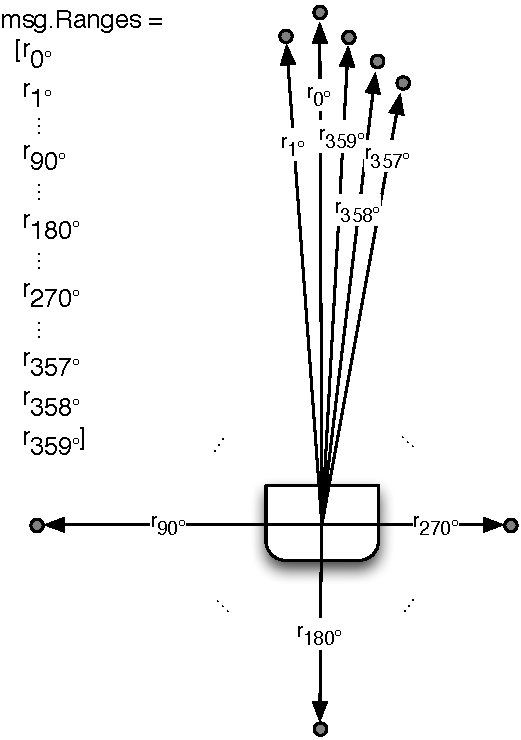
\includegraphics[width=2.0in]{figs/laserscanmessage}
\caption{A schematic of the laser scan data.  In the figure, $r_{\theta^\circ}$ indicates the distance in meters to a detected object at a bearing of $\theta$ degrees.   $msg.Ranges$ shows how each of these distances maps to a particular index in the array.  The array holds the distances, and the angles are implicitly encoded by the position in which they appear in the array.  If no detection is made at a particular bearing, the value $0.0$ is used instead.  Note: the angles of the measurements around $\theta = 0^\circ$ have been exaggerated for visualization purposes (i.e. the angles shown are larger than a single degree).\label{fig:laserscanmessage}}
\end{marginfigure}



Sometimes it is useful to take the raw points detected by the laser scanner and interpret them as geometrical objects (e.g., lines, curves, polygons).  For instance, given the laser scan in Figure \ref{fig:scanexample} we may wish to automatically interpret the laser scan data (i.e. pick out lines, circles, etc.).  In the context of the present challenge, the ability to differentiate between lines and circles is crucial to running The Gauntlet\texttrademark  since walls are obstacles and the circle denotes the goal.
\begin{figure}
\begin{center}
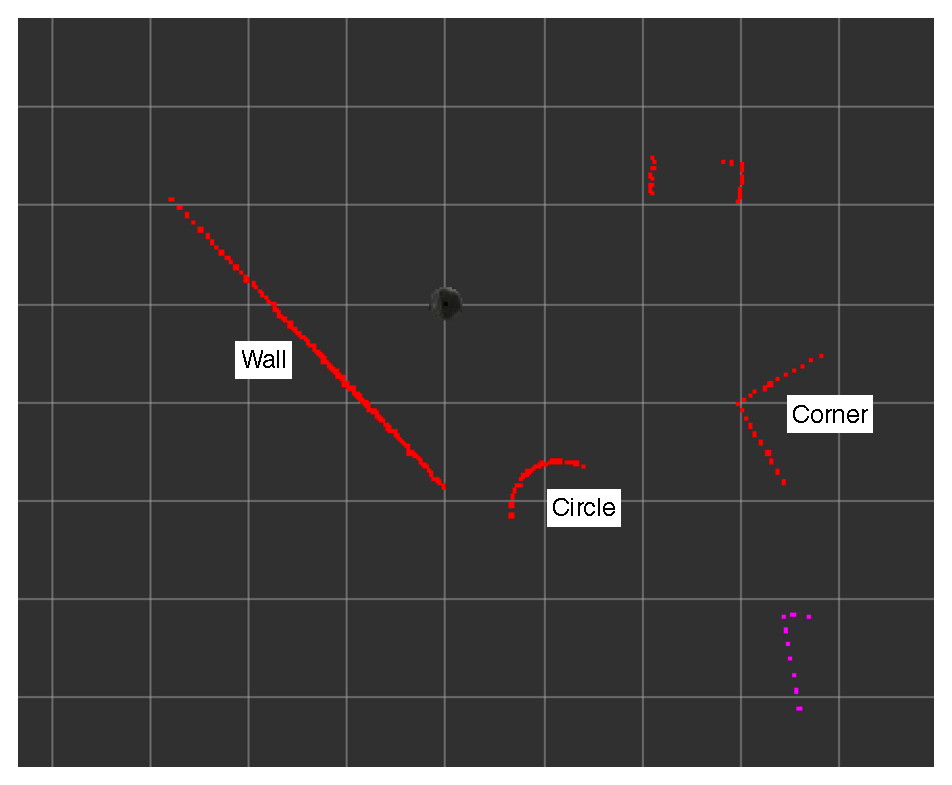
\includegraphics[width=.8\linewidth]{figs/playgroundscan}
\end{center}
\caption{A laser scan with high-level features identified.\label{fig:scanexample}}
\end{figure}

Conveniently, in modules 1 and 2 we've built a lot of the machinery needed to do just this (aren't we sneaky?).  Here, you'll have a chance to bring it all together.

\subsection{It's like your birthday, but way better! [1 hr]}

Today you get to play with a new sensor, and that's awesome! Before you start using the Neato's LIDAR to do really interesting and useful things, it is important to take a few minutes to understand the sensor's characteristics and limitations. Typically you would approach understanding the capabilities of a new sensor by first reading the relevant data sheets and manuals (I know, not really in the typical engineering playbook), then conducting some simple characterization experiments. For this assignment, let's assume the section above where the LIDAR was introduced and the approximate range and angular resolution of the sensor were given was the data sheet. Congratulations, you read the data sheet!


\vspace{0.5cm}

\begin{enumerate}[series=exercises, label=\textbf{Exercise} (\arabic*)]

\item Now, think about some simple experiments you could perform to learn more about the LIDAR. You can do these using the ``teleopAndVisualizer'' function to visualize the LIDAR data. Listed below are some suggestions for questions to answer about the LIDAR, but don't feel limited! You don't need to spend much more than an hour on this, we just want you to get a good feel for the LIDAR. You should make note of the question you wanted to answer, the experiment you ran, the results, and what you learned about the LIDAR.
%\paragraph{Exercise 3}
\begin{enumerate}
\item What is the maximum range of the LIDAR? Does it match the spec given above? Does this range vary with environmental conditions?

\item Does the type of surface impact the LIDAR measurement? Matte or glossy? Glass?

\item Does the angle of a surface impact the LIDAR measurement?

\item Does the LIDAR have a minimum distance or dead-zone around the sensor? What are the implications of this if so?

\item How does light impact the LIDAR? Sunlight? Dark?

\item What is the minimum object size that can be detected? How does this relate to the angular resolution?
\end{enumerate}
\end{enumerate}
\solution{Experiments and answers to this question may vary. The goal is to develop an understanding of the performance and limitations of the LIDAR sensor. This is important when creating experimental protocols,  identifying bad measurements in a data set, or deciding on a sensor to purchase/use for a given application. Generally LIDAR has trouble with glass and bright sunlight. It should work great in the dark. It seems that the LIDAR on the NEATO has a dead zone around the robot, but it is hard to determine if that is due to the sensor or if measurments within a certain distance are simply rejected in software. }


\begin{marginfigure}

\includegraphics[width=2in]{figs/sensor}
\caption{Can't argue with this one.}
\end{marginfigure}

\subsection{Polar and Cartesian Coordinates [1 hr]}
LIDAR data and indeed data in many other applications are typically presented in polar coordinates. In many other situations however, it is more convenient to represent the data in Cartesian coordinates. In this set of exercises, you will get some practice converting polar to Cartesian coordinates and vice-versa.

In a point in 2-D space can be described as a sum of unit vectors in the $\hat{\mathbf{i}}$ and $\hat{\mathbf{j}}$ directions which are unit vectors in the directions of the $x$ and $y$ axes respectively.

\begin{figure}
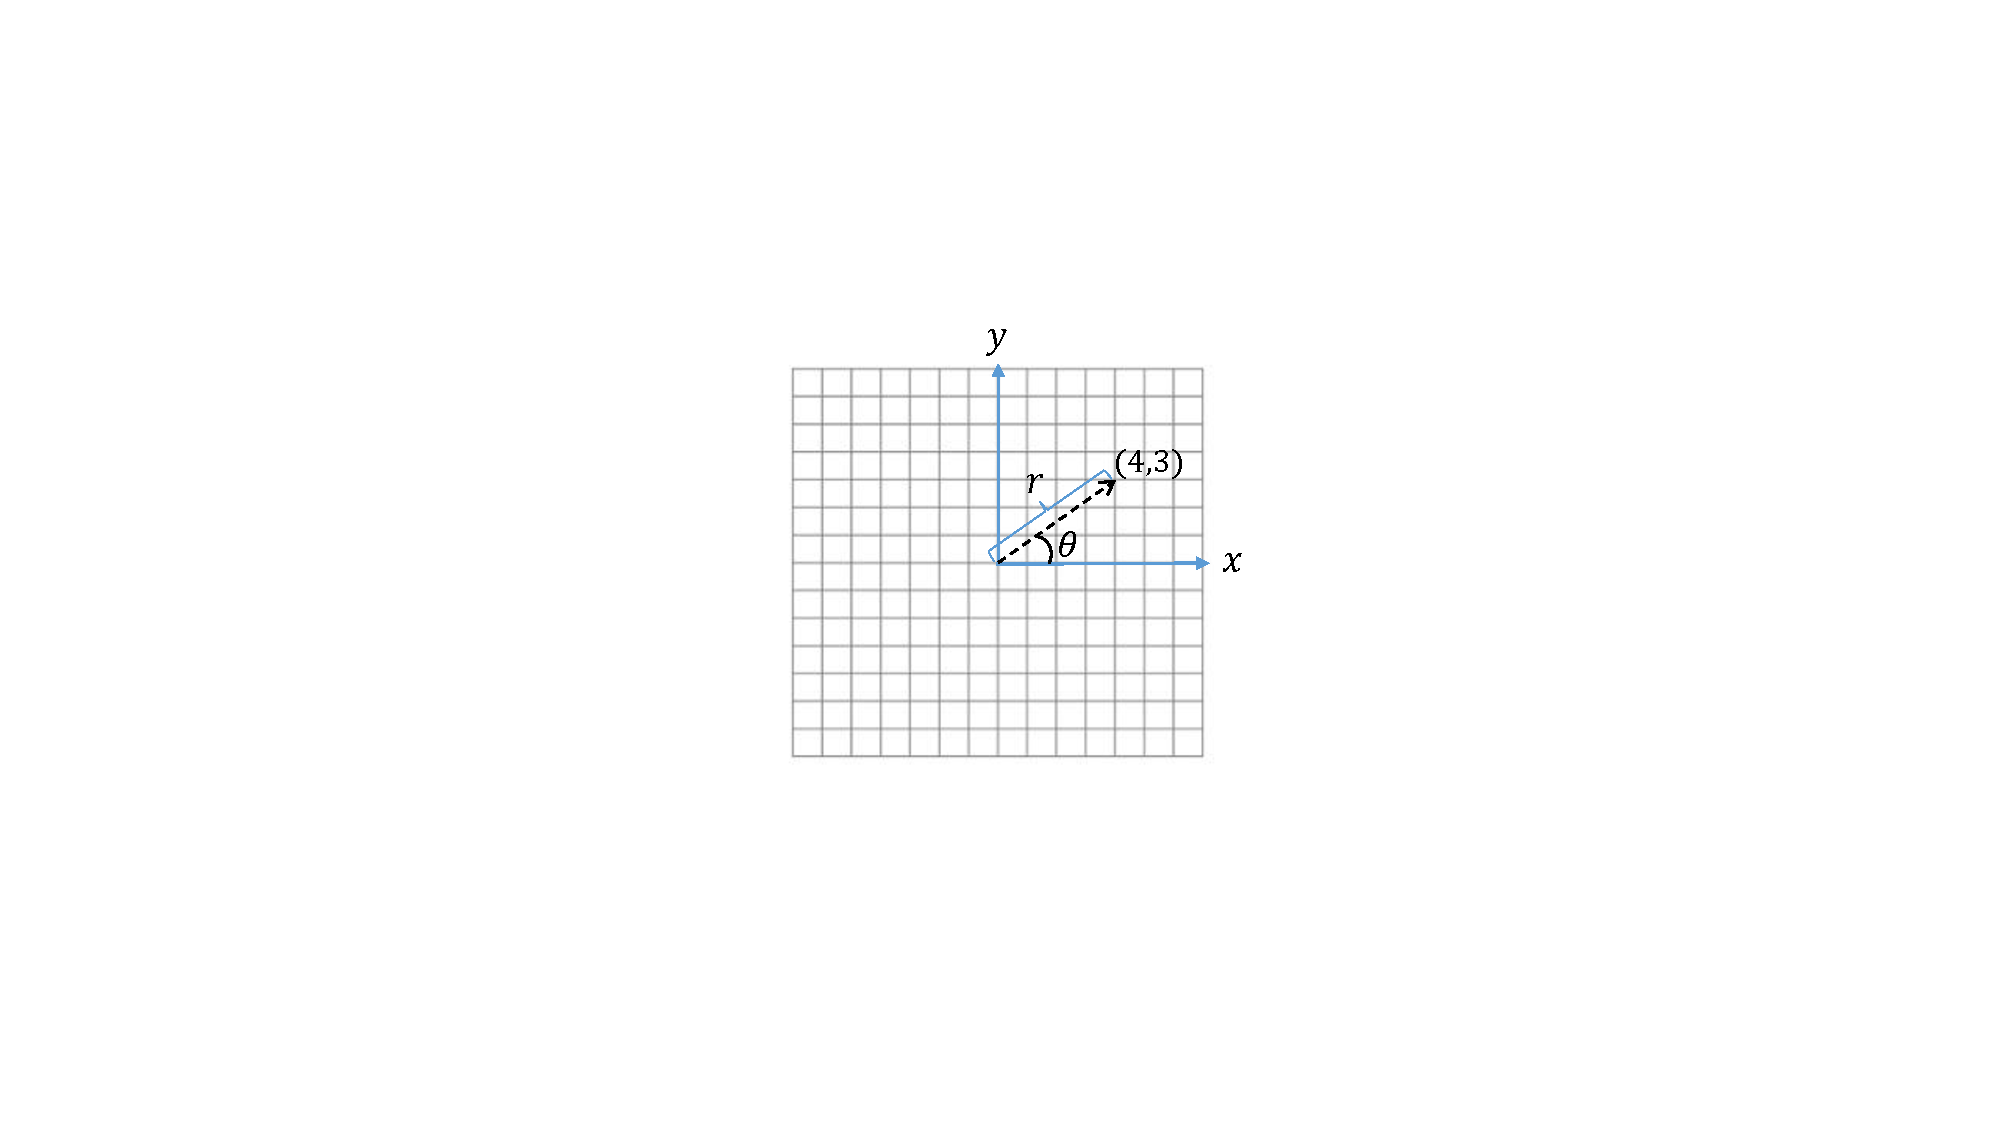
\includegraphics[width=3in]{figs/PolarCartesianVector43.pdf}
\caption{Illustration of vector in polar and Cartesian coordinates.}
\label{fig:VecRotation}
\end{figure}

Consider the point $(4,3)$ illustrated in Figure \ref{fig:VecRotation}.  You can write the vector representing this point as a sum of $\hat{\mathbf {i}}$ and $\hat{\mathbf{j}}$ as follows
\begin{align}
\twobyone{4}{3} = 4\hat{\mathbf{i}} + 3\hat{\mathbf{j}}
\end{align}
We can also write this point in terms of polar co-ordinates as $(r, \theta)$, where
\begin{align}
r &= \sqrt{4^2+3^2} = 5\\
\theta &= \tan^{-1}\left(\frac34\right)
\end{align}

In general a vector $(x,y)$ in Cartesian coordinates can be expressed in polar coordinates as $(r,\theta)$ where
\begin{align}
r &= \sqrt{x^2 + y^2}\\
\theta &= \tan^{-1}\left(\frac{y}{x}\right)
\end{align}

To go from polar to cartesian coordinates, we can use the following formulas

\begin{align*}
x &= r\cos \theta\\
y &= r\sin \theta
\end{align*}

Besides expressing a vector as a linear combination of the $\hat{\mathbf{i}}$ and $\hat{\mathbf{j}}$ vectors, we can also define two new unit vectors $\hat{\mathbf{r}}$ and $\hat{\boldsymbol{\theta}}$ defined as follows
\begin{align}
\hat{\mathbf{r}}   &= \twobyone{\cos \theta}{\sin \theta}\\
\hat{\boldsymbol{\theta}}  &= \twobyone{-\sin \theta}{\cos \theta}
\end{align}
Note that these vectors are not absolute with respect to the origin of the cartesian coordinates. While it does seem strange to represent unit vectors in this manner, this kind of representation will prove useful in the near future when we are dealing with dynamics of rotating bodies (i.e. you will not directly use this until next semester, but we thought we should give you a preview).
\vspace{1em}
\begin{enumerate}[resume=exercises, label=\textbf{Exercise} (\arabic*)]

\item Convert the following from Cartesian to polar coordinates.
\be
\item $(x,y) = \left(-8, 6\right)$
\solution{$\theta$=2.5 radians, R=10}
\item $(x,y) = \left(5, 12\right)$
\solution{$\theta$=1.18 radians, R=13}
\ee


\item Convert the following from polar to Cartesian coordinates.
\be
\item $(r, \theta) = \left(2, \frac{\pi}{6}\right)$
\solution{x=1.73, y=1.00}
\item $(r, \theta) = \left(2, -\frac{\pi}{3}\right)$
\solution{x=1, y=-1.73}
\ee



\item What is $\hat{\mathbf{r}}^T \, \hat{\boldsymbol{\theta}} $?
\solution{$\hat{r}$ and $\hat{\theta}$ are orthogonal, so $\hat{r}^{T} \hat{\theta}$=0.}

\item In words, describe the $\hat{\mathbf{r}}$ and $\hat{\boldsymbol{\theta}}$ vectors.
\solution{The $\hat{r}$ vector has length 1 and points in the direction of $\vec{r}$, and $\hat{\theta}$ has length 1 and points in the direction of increasing $\theta$, orthogonal to $\hat{r}$.}


\item Write the following points in terms of the $\hat{\mathbf{r}}$ and $\hat{\boldsymbol{\theta}}$ vectors
\be
\item $(4,3)$.
\solution{This was a very poorly worded problem and was not graded.}
\item $\left(3, \frac{\pi}{3}\right)$
\ee

\item Now let's look at some LIDAR data that was collected from the Chamber of Emptiness\texttrademark, which is a desolate room with one wall. Load the data in \textit{scan1.mat}, which should contain the variables \textit{r} for range (distance from the scanner in meters) and \textit{theta} for the angle from the front of the robot (see Figure~\ref{fig:scanexample}).
\be
\item Plot these data using: \begin{verbatim} plot(theta,r,'ks')\end{verbatim}
\solution{\begin{figure}
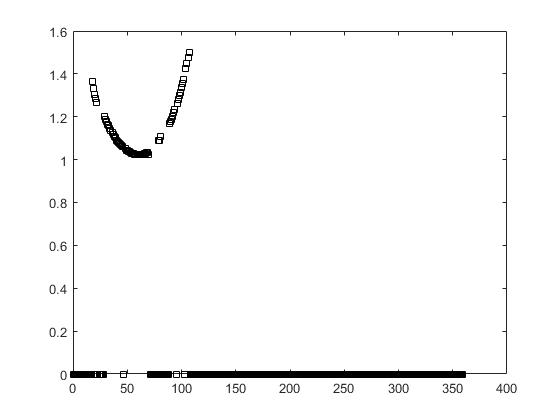
\includegraphics[width=4in]{figs/7a}
\caption{Answer for 7a.}
\end{figure}
\clearpage}

\item Plot the data in polar coordinates using:
\begin{verbatim}	polarplot(deg2rad(theta),r,'ks',...
   'MarkerSize',6,'MarkerFaceColor','m')
\end{verbatim}

\solution{\begin{figure}
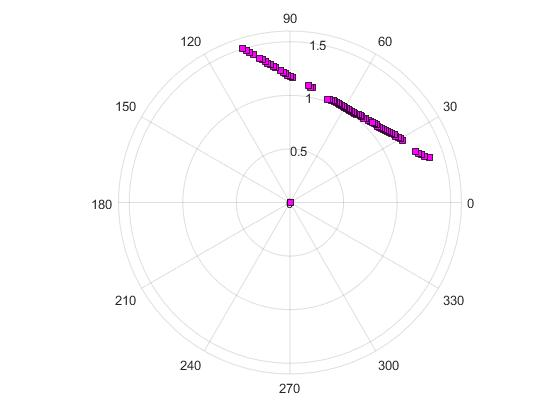
\includegraphics[width=4in]{figs/7b}
\caption{Answer for 7b.}
\end{figure}}

\item You should see two subsets of data (a line and a parabola in the plot from part a). Where are these two subsets represented in the polarplot?
\solution{The samples making up the line in part a are all at zero distance, and appar as a cluster and the center of the polar plot. The parabola from part a becomes the line in part b.}

\item When the LIDAR does not detect any object at a given angle, it outputs a 0 for the value of \textit{r} at that angle (this is a common problem in the Chamber of Emptiness). Create new variables \textit{theta\_clean} and \textit{r\_clean} which represent the angles and values of \textit{r} when \textit{r} is not zero.
\solution{one implementation:\\
index=find(r$\sim$ =0); \\
r\_clean=r(index);\\
theta\_clean=theta(index);

\begin{figure}
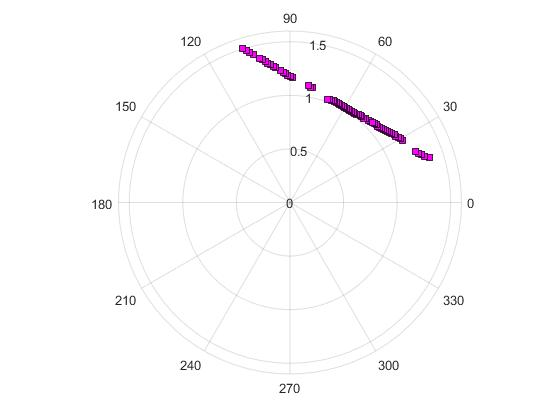
\includegraphics[width=4in]{figs/7d}
\caption{Answer for 7d.}
\end{figure}}

\item Now convert \textit{r\_clean} and \textit{theta\_clean} to Cartesian coordinates and plot them using the \textit{plot()} function.

\solution{\begin{figure}
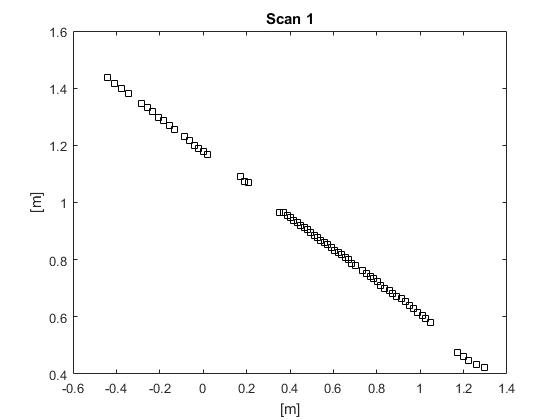
\includegraphics[width=4in]{figs/7e}
\caption{Answer for 7e.}
\end{figure}}

\ee
\ee
% scan1 diagonal in r and theta will zeros for r values

\section{Fitting Models to Laser Scan Data [3 hours]}


\subsection{Least Squares for Line Fitting}
The first structure we would like to detect in the laser scan data is a line.  We've seen the notion of a line of best fit a couple of times in Module 2.  The first time we saw it was when we studied linear regression.
For instance, during Day 5 in module 2 you used the temperatures of Boston, Providence, and Washington D.C. to predict the temperature in New York.  This lead to the following model for predicting the temperature in New York on day $i$: $\hat{T}_N(i) = \beta_3 T_W(i) + \beta_2 T_B(i) + \beta_1 T_P(i) + \beta_0$.  This model gave rise to the following equation for MSE.
\begin{align}
MSE(\beta_0, \beta_1, \beta_2, \beta_3) &= \frac{1}{n}\sum_{i=1}^n \left ( T_N(i) - \hat{T}_N(i) \right)^2  \nonumber \\
MSE(\beta_0, \beta_1, \beta_2, \beta_3) &= \frac{1}{n}\sum_{i=1}^n \left ( T_N(i)  - ( \beta_3 T_W(i) + \beta_2 T_B(i) + \beta_1 T_P(i) + \beta_0) \right)^2 \label{eq:MSEtemperature}
\end{align}

In the previous section, we converted each detection in our laser scan data into Cartesian coordinates.  Let's call this set of points $(x_1, y_1), (x_2, y_2), \ldots, (x_n, y_n)$.  Further, let's assume that the relationship between $x$ and $y$ is given by $y = \beta_1 x + \beta_0 + \epsilon$ (where $\epsilon$ is an error term that we'd like to minimize).
%\todo[size=\small]{I cut the eqs for slope and offset to make them go back to their module 2. Should I add this back in to help them out? Or leave it out to help them make the connection to what they did before?}

%$y = ax + b + \epsilon$ (where $\epsilon$ is an error term that we'd like to minimize).  Using the mathematics that you learned when we studied linear regression, we can write an expression for the values of $a$ and $b$ that minimize the mean squared error.
%\begin{align}
%a &= \frac{\sum_{i=1}^n \left ( x_i - \mu_x \right ) \left ( y_i - \mu_y \right )}{\sum_{i=1}^n \left ( x_i - \mu_x \right )^2} \nonumber \\
%b &= \mu_y - a\mu_x \nonumber
%\end{align}
%Where $\mu_x$ and $\mu_y$ stand for the mean of x and y respectively.



%\paragraph{Exercise 3}
\begin{quote}Desired learning outcomes:
\bi
\item Increase proficiency in coding solutions to linear regression problems.
\item Draw connections to previous work in this class.
\item Determine conditions under which an algorithm is ill-suited for application.
\ei
\end{quote}
\begin{enumerate}[resume=exercises, label=\textbf{Exercise} (\arabic*)]
\setcounter{enumi}{6}
\item Find the linear regression line of best fit (values of $\beta_0$ and $\beta_1$) for the Cartesian representation of the laser scan from \emph{scan1.mat}.  Plot the line of best fit.  Save your values for the line of best fit; you will recreate this again later to compare against another method. It may be helpful to revisit your work from Module 2, Day 4 and Night 4;  Module 2, Day 5; and/or your smile detection code.

\solution{\begin{figure}
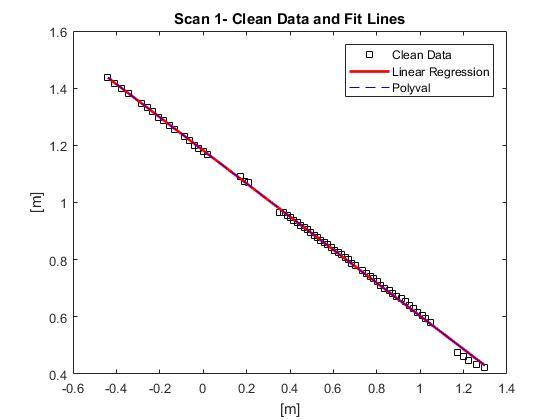
\includegraphics[width=4in]{figs/Scan1_fits}
\caption{Clean data and best fit lines using linear regression and the Matlab Polyfit function for Scan 1.}
\end{figure}}

\item Repeat Exercises 6d-e and 7 for \emph{scan2.mat}, \emph{scan3.mat}, and \emph{scan4.mat}.
\solution{\begin{figure}
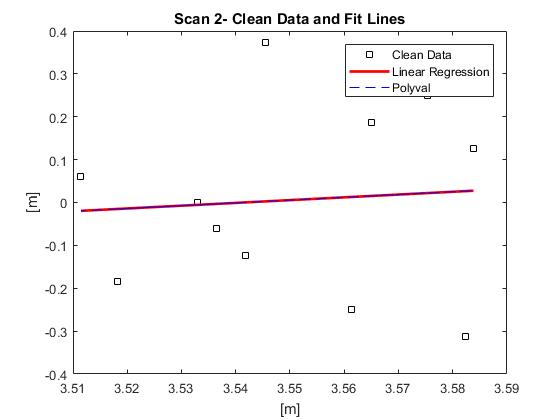
\includegraphics[width=4in]{figs/Scan2_fits}
\caption{Clean data and best fit lines using linear regression and the Matlab Polyfit function for Scan 2.}
\end{figure}
\begin{figure}
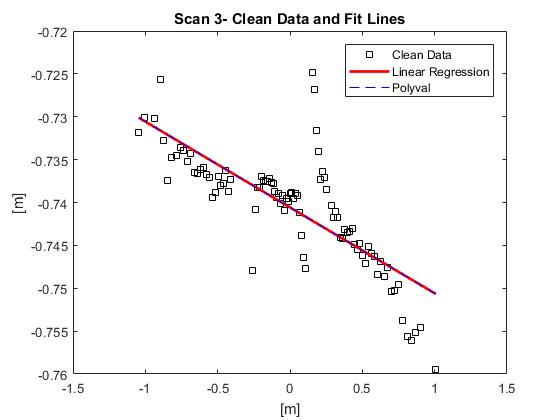
\includegraphics[width=4in]{figs/Scan3_fits}
\caption{Clean data and best fit lines using linear regression and the Matlab Polyfit function for Scan 3.}
\end{figure}
\begin{figure}
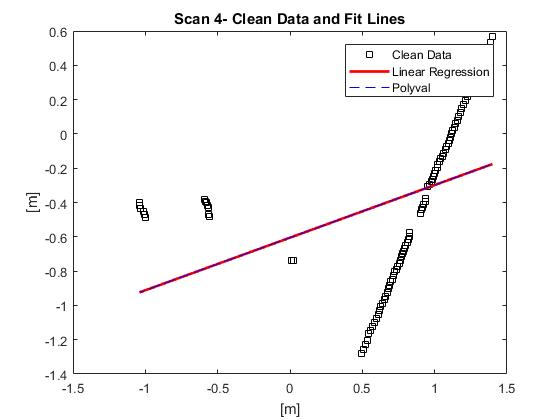
\includegraphics[width=4in]{figs/Scan4_fits}
\caption{Clean data and best fit lines using linear regression and the Matlab Polyfit function for Scan 4.}
\end{figure}}
\item Note what you observe, and comment on any deficiencies with this approach to line fitting.
\solution{Most apparent deficiency is that linear regression is skewed by the presence of outliers in the dataset.}

%\item Load the two datasets \emph{scan1.mat} and \emph{scan2.mat}.  Each contains the Cartesian representation of two laser scans.  For each scan, compute the line of best fit (values of $a$ and $b$) using the formulas given above.  Plot the line of best fit for each scan, and include these plots in your writeup.  In comparing the results on the two scans, comment on any deficiencies with this approach to line fitting.

\ee


% scan2 regular vertical line at a distance

\subsection{Principal Component Analysis [3 hr]}

Linear regression defines the line of best fit in terms of the sum of squared distances, measured vertically, between the data points and the line (see Figure~\ref{fig:differentobjectives}).  However, when determining the best fitting line for a laser scan, there's nothing special about the vertical direction.  In fact, it would make as much sense to minimize the sum of the squared horizontal distances.  In this context, a much more natural way to think about the line of best fit is to minimize the perpendicular distances between the line and the data points (see Figure~\ref{fig:differentobjectives}).
\vspace{1 em}
\begin{quote}Desired learning outcomes:
\bi
\item Generalize knowledge of an algorithm you've already learned by applying it in a new context.
\item Plot lines that are defined parametrically.
\item See the connection between different objective functions and the resultant optimal solutions.
\ei
\end{quote}
\begin{enumerate}[resume=exercises, label=\textbf{Exercise} (\arabic*)]


\item Think about how to use principal component analysis to determine the line of best fit that minimizes the sum of squared perpendicular distances as shown by the blue dashed lines in Figure~\ref{fig:differentobjectives}.
\be
\item Describe conceptually why you think this algorithm will achieve the desired goal.
\solution{We can recall from Module 2 Night 7 that PCA identifies the direction of greatest variation in a data set (this direction is given by the eigenvector associated with the largest eigenvalue). Conceptually, the direction of \emph{greatest} variation should be orthogonal to the direction of \emph{least} variation. So, the direction perpendicular, or orthogonal, to the line found using PCA should minimize variation, and therefore minimize the sum of squared perpendicular distances.}

\item Write pseudocode to describe the steps you will need to take. You should consider what an eigenvector represents. (Hint: if you translate your data, be sure to translate it back. )
\solution{
\begin{enumerate}
\item Convert data from polar to cartesian coordinates.
\item Calculate the x and y means for the dataset.
\item Use the x and y means to center the data.
\item Find the singular value decompositon (SVD).
\item Identify the direction of greatest variation in the dataset as the eigenvector associated with the largest eigenvalue.
\item Translate the data back to its original positions.
\ee}
\ee
\item In MATLAB, do the following for the Cartesian data from each of the four scans \emph{scan1.mat}, \emph{scan2.mat}, \emph{scan3.mat} and \emph{scan4.mat}.  % scan 1 is diag, 2 is vert, 3 is horiz, 4 is another diag with a few outliers
\be
\item Compute the line of best fit using PCA.
\item Plot the data points, line of best fit from PCA, and line of best fit from linear regression. Be sure to note which line is which.
\solution{
\begin{figure}
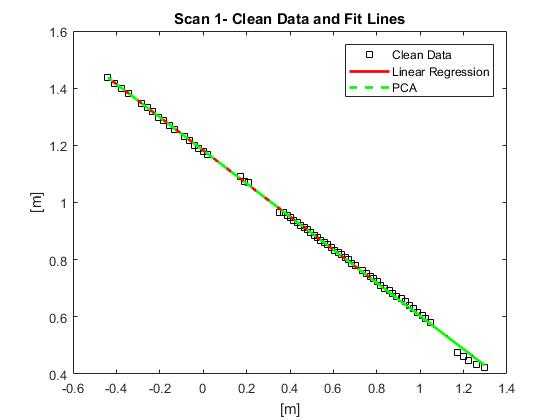
\includegraphics[width=4in]{figs/Scan1_pca}
\caption{Clean data and best fit lines using linear regression and PCA for Scan 1.}
\end{figure}
\begin{figure}
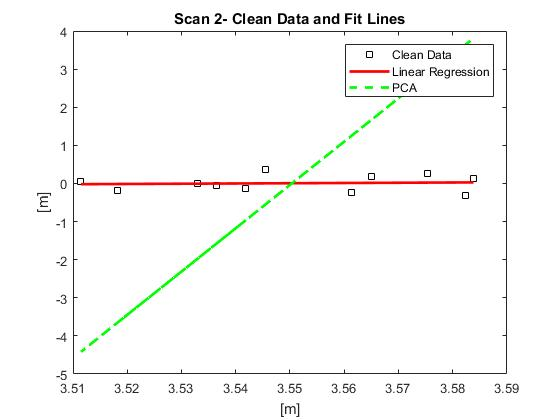
\includegraphics[width=4in]{figs/Scan2_pca}
\caption{Clean data and best fit lines using linear regression and PCA for Scan 2.}
\end{figure}
\begin{figure}
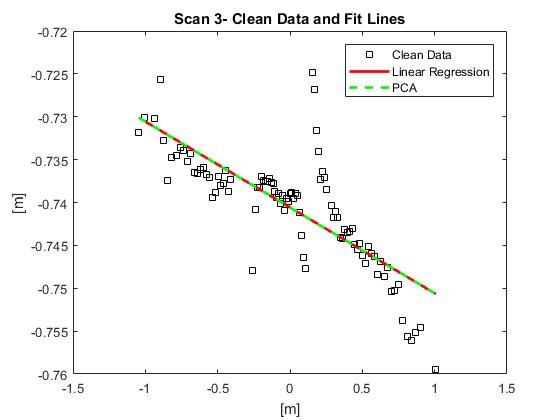
\includegraphics[width=4in]{figs/Scan3_pca}
\caption{Clean data and best fit lines using linear regression and PCA for Scan 3.}
\end{figure}
\begin{figure}
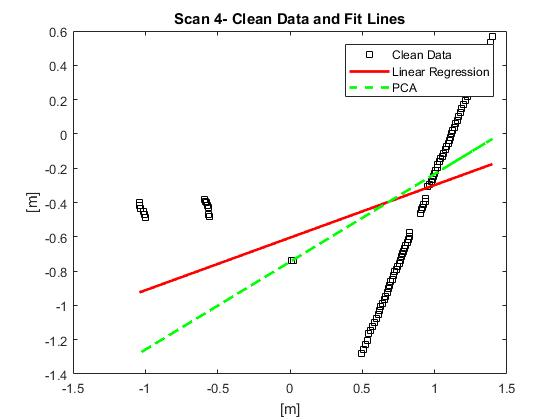
\includegraphics[width=4in]{figs/Scan4_pca}
\caption{Clean data and best fit lines using linear regression and PCA for Scan 4.}
\end{figure}}
\item Comment on the differences between the fits for each data set.
\ee
\ee

\begin{marginfigure}
\begin{center}
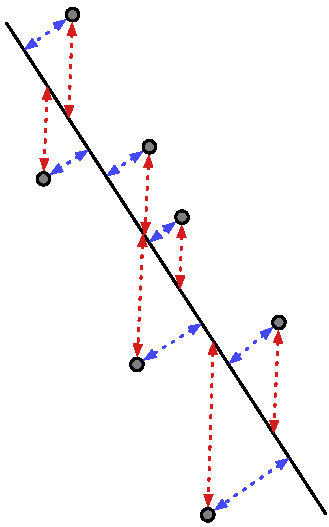
\includegraphics[width=1.5in]{figs/differentbestfits}
\end{center}
\caption{Laser scan points (gray dots), a proposed fitted line, and two different notions of error.  The red dashed lines provide the vertical distance (which is used in linear regression).  The blue dashed lines provide the perpendicular distance which is a more natural way to define line of best fit in the context of fitting lines to laser scan data.\label{fig:differentobjectives}}
\end{marginfigure}



\end{document}
